%%%%%%%%%%%%%%%%%%%%%%%%%%%%%%%%%%%%%%%%%%%%%%%%%%%%%%%%%%%%%%%%%%%%
%% I, the copyright holder of this work, release this work into the
%% public domain. This applies worldwide. In some countries this may
%% not be legally possible; if so: I grant anyone the right to use
%% this work for any purpose, without any conditions, unless such
%% conditions are required by law.
%%%%%%%%%%%%%%%%%%%%%%%%%%%%%%%%%%%%%%%%%%%%%%%%%%%%%%%%%%%%%%%%%%%%

\documentclass[
  digital, %% This option enables the default options for the
           %% digital version of a document. Replace with `printed`
           %% to enable the default options for the printed version
           %% of a document.
  twoside, %% This option enables double-sided typesetting. Use at
           %% least 120 g/m² paper to prevent show-through. Replace
           %% with `oneside` to use one-sided typesetting; use only
           %% if you don’t have access to a double-sided printer,
           %% or if one-sided typesetting is a formal requirement
           %% at your faculty.
  notable,   %% This option causes the coloring of tables. Replace
           %% with `notable` to restore plain LaTeX tables.
  nolof,   %% This option prints the List of Figures. Replace with
           %% `nolof` to hide the List of Figures.
  nolot,   %% This option prints the List of Tables. Replace with
           %% `nolot` to hide the List of Tables.
  %% More options are listed in the user guide at
  %% <http://mirrors.ctan.org/macros/latex/contrib/fithesis/guide/mu/fi.pdf>.
]{fithesis3}
%% The following section sets up the locales used in the thesis.
\usepackage[resetfonts]{cmap} %% We need to load the T2A font encoding
\usepackage[T1,T2A]{fontenc}  %% to use the Cyrillic fonts with Russian texts.
\usepackage[
  main=slovak,  %% By using `czech` or `slovak` as the main locale
                %% instead of `english`, you can typeset the thesis
                %% in either Czech or Slovak, respectively.
  %english, german, russian, czech, slovak %% The additional keys allow
]{babel}        %% foreign texts to be typeset as follows:
%%
%%   \begin{otherlanguage}{german}  ... \end{otherlanguage}
%%   \begin{otherlanguage}{russian} ... \end{otherlanguage}
%%   \begin{otherlanguage}{czech}   ... \end{otherlanguage}
%%   \begin{otherlanguage}{slovak}  ... \end{otherlanguage}
%%
%% For non-Latin scripts, it may be necessary to load additional
%% fonts:
\usepackage{paratype}
\def\textrussian#1{{\usefont{T2A}{PTSerif-TLF}{m}{rm}#1}}
%%
%% The following section sets up the metadata of the thesis.
\thesissetup{
    date          = \the\year/\the\month/\the\day,
    university    = mu,
    faculty       = fi,
    type          = mgr,
    author        = Bc. Ondrej Oravčok,
    gender        = m,
    advisor       = {RNDr. Radek Ošlejšek, Ph.D.},
    title         = {Interaktívna časová os ako modul v Angulare},
    %TeXtitle      = {The Proof of $\mathsf{P}=\mathsf{NP}$},
    TeXtitle      = {Interaktívna časová os ako modul v Angulare},
    keywords      = {keyword1, keyword2, ...},
    TeXkeywords   = {keyword1, keyword2, \ldots},
    abstract      = {This is the abstract of my thesis, which can

                     span multiple paragraphs.},
    thanks        = {These are the acknowledgements for my thesis, which can

                     span multiple paragraphs.},
    %bib           = prace.bib,
}
\usepackage{makeidx}      %% The `makeidx` package contains
\makeindex                %% helper commands for index typesetting.
%% These additional packages are used within the document:
\usepackage{paralist} %% Compact list environments
\usepackage{amsmath}  %% Mathematics
\usepackage{amsthm}
\usepackage{amsfonts}
\usepackage{url}      %% Hyperlinks
\usepackage{markdown} %% Lightweight markup
\usepackage{listings} %% Source code highlighting
\lstdefinelanguage{TypeScript}{
    morekeywords={number, string, object,
        typeof, let, public, private, void
        },
    sensitive=false, % keywords are not case-sensitive
    morecomment=[l]{//}, % l is for line comment
    morecomment=[s]{/*}{*/}, % s is for start and end delimiter
    morestring=[b]' % defines that strings are enclosed in double quotes
}
\lstset{
%  basicstyle      = \ttfamily,%
%  identifierstyle = \color{black},%
%  keywordstyle    = \color{blue},%
%  keywordstyle    = {[2]\color{cyan}},%
%  keywordstyle    = {[3]\color{olive}},%
%  stringstyle     = \color{teal},%
%  commentstyle    = \itshape\color{magenta}}
  language=TypeScript,
  aboveskip=3mm,
  belowskip=3mm,
  showstringspaces=false,
  columns=flexible,
  basicstyle={\small\ttfamily},
  numbers=left,
  xleftmargin=1.25em,
  numberstyle=\tiny\color{gray},
  keywordstyle=\color{blue},
  commentstyle=\color{darkgray},
  stringstyle=\color{olive},
  breaklines=true,
%  breakatwhitespace=true,
%  tabsize=3
}
\usepackage{floatrow} %% Putting captions above tables
\floatsetup[table]{capposition=top}
\usepackage[backend=biber,sorting=none]{biblatex}
\addbibresource{prace_mgr.bib}
\usepackage{graphicx}
\graphicspath{ {pics/} }

\begin{document}
\chapter*{Úvod}
\addcontentsline{toc}{chapter}{Introduction}
Toto bude úvod.

\chapter{Kybernetický polygón}
Podľa Národného bezbečnostného úradu Českej republiky je termínom \textit{kritická informačná infraštruktúra} označený \textit{"systém prvkov tejto infraštruktúry, ktorý pri narušení svojej funkcie môže spôsobiť poškodenie alebo ohrozenie záujmov Českej republiky"}\cite{nbu2012}.

Kybernetický polygón (KYPO) bol zriadený Ministerstvom vnútra Českej republiky za účelom zaistenia kybernetickej bezpečnosti v Českej republike ochranou kritickej informačnej infraštruktúry. Projekt KYPO poskytuje unikátne prostredie pre výskum nových metód, ktoré by v blízkej budúcnosti mohli pomôcť chrániť kritickú informačnú infraštruktúru\cite{dankovvcikova2015konfigurace}. Objekt polygónu bol vybudovaný v roku 2015 vrámci rekonštrukcie Fakulty Informatiky.
%V rýchlo sa rozvíjajúcom svete informačných technológií je informačná bezpečnosť najdôležitejším odvetvím informatiky. V dnešnej dobe už nie je veľmi pravdepodobné, aby nás výdobytky techniky ako telefóny a počítače ohrozovali na živote. Hrozba informačnej bezpečnosti sa týka hlavne ochrany informácií. Masarykova Univerzita si uvedomuje vážnosť tejto hrozby a preto sa rozhodla zriadiť výzkumné stredisko v tejto oblasti.

\section{Technológie}
Toto prostredie funguje na princípe cloudového riešenia v ktorom je možné modelovať virtuálnu sieť\cite{eichler2014analytical}. Toto riešenie poskytuje všetky nástroje potrebné k simulácii rôznych sieťových topológií. Prostredie je určené pre výzkum a testovanie rôznych scenárov kybernetických útokov v izolovanom a plne kontrolovateľnom prostredí\cite{vceleda2015kypo}.

\section{Architektúra}
Prostredie kybernetického polygónu je implementované ako cloudové riešenie modelu Platform as a Service. Obrázok \ref{kypo_structure} znázorňuje jednotlivé vrstvy architektúry:

\begin{description}
\item[Users] - užívatelia s rôznymi skúsenosťami môžu interagovať buď cez Portál alebo priamo s niektorou nižšou vrstvou
\item[Portal] - Portál je grafické používateľské rozhranie (GUI), ktoré v prípade KYPO využíva portálový server Liferay opísaný v kapitole~\ref{liferay}
\item[Scenario and sandbox management API] slúži na konfiguráciu, vytváranie, editovanie a likvidáciu sandboxov. Sandbox je izolovaný súbor virtuálnych strojov a sieťovej konfigurácie, ktorý užívateľovi poskytuje kľúčovú funkcionalitu ako napríklad možnosť opakovať a modifikovať experiment.
\item[Monitoring API] umožňuje monitorovanie sieťových prepojení a konfigurácie uzlov. Komunikuje buď s OpenNebula alebo priamo s existujúcimi virtuálnymi inštanciami.
\item[Cloud API] slúži ako univerzálne rozhranie pre vyššie vrstvy ktoré abstrahuje od konkrétnej implementácie IaaS\footnote{Infrastructure as a Service} nižších vrstiev, aby bola zabezpečená flexibilita cloudového riešenia.
\item[OpenNebula platform] - IaaS - umožňuje manažment rôznorodých výpočtových kapacít (najčastejšie virtualizovaných) a spadá pod správu CERIT Scientific Cloud
\item[Computing infrastructure] zahrňuje fyzické objekty, sieťové prvky a všetok potrebný hardvér ktorý poskytuje pamäť a výpočtovú silu.
\end{description}

\begin{figure}
	\center
	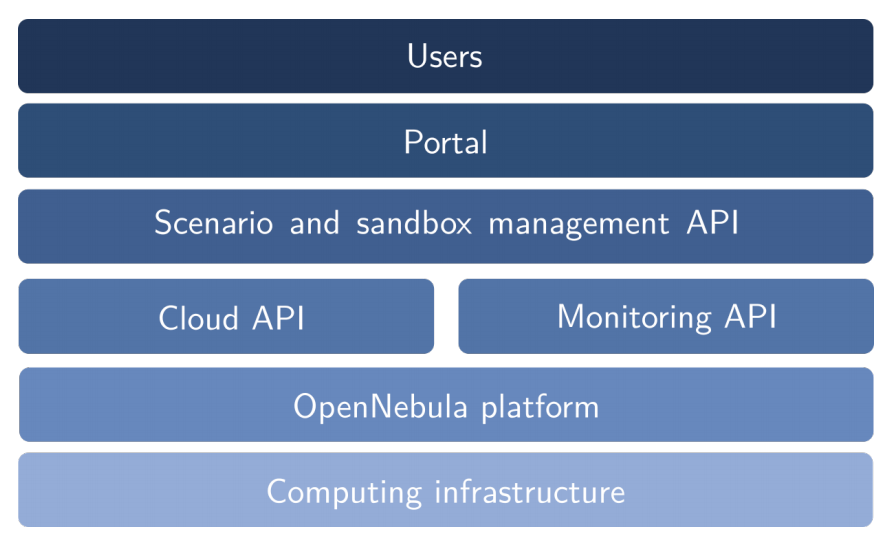
\includegraphics[width=1.0\linewidth]{kypo_structure}
	\caption{Architektúra cloudového riešenia KYPO\cite{vceleda2015kypo}}
	\label{kypo_structure}
\end{figure}

\section{Potreba analýzy dát}
Nakoľko simulácie útokov a cvičenia prebiehajú v reálnom čase, vznikla potreba sledovať zmeny v týchto dynamických prostrediach. Priebehy jednotlivých scenárov sa zaznamenávajú aj pre potreby neskoršej analýzy. Portlet časovej osy slúži ako kľúčový element pre filtrovanie týchto dát, či už sa jedná o analýzu starších dát, alebo sledovanie aktuálne pribúdajúcich dát v reálnom čase.

\chapter{Liferay Portal}
\label{liferay}
V kontexte webových aplikácií môžeme portál definovať\cite{sezov2011liferay} ako \textit{"Samostatne oddelené webové prostredie, z ktorého sú spustiteľné všetky aplikácie užívateľa. Tieto aplikácie sú systematicky integrované na jednom mieste."}

Liferay je portálový server distribuovaný pod licenciou LGPL, v ktorom je zmysluplne umožnená spolupráca a zdieľanie informácií rôznym používateľom. Umožňuje vykonávať správu obsahu pomocou WYSIWYG\footnote{WYSIWYG - \textit{what you see is what you get} teda \textit{"to, čo vidíš je to, čo aj dostaneš"} je spôsob práce s grafickým rozhraním, pri ktorom sa kód (najčastejšie HTML) generuje na základe našich predstáv, pričom do neho vôbec priamo nezasahujeme} editora. Používateľ tak nepotrebuje žiadnu hlbokú znalosť HTML ani iného programovacieho jazyka. Jednotlivé komponenty stránky si vie jednoducho prispôsobiť a výsledok vidí vždy okamžite\cite{sezov2011liferay}.

Portálový server Liferay je naprogramovaný v jazyku Java, preto na jeho beh potrebujeme aplikačný server, alebo aspoň servlet kontajner. Liferay natívne podporuje napríklad Apache Tomcat, GlassFish, JBoss, WebLogic, WebSphere a mnoho ďalších.

\section{Používatelia}
\label{liferay_users}
Do portálov majú prístup užívatelia (Users), ktorý môžu byť priraďovaný do skupín (User Groups). Užívatelia taktiež môžu byť priraďovaný do organizácií (Organizations). Tieto organizácie sú zoskupované do rôznych hierarchických štruktúr, popri ktorých ešte v Liferay existujú komunity (Communities) a tímy (Teams). Detailnejší náhľad do štruktúry nám poskytne obrázok \ref{liferay_structure}.

Liferay tak v tomto smere poskytuje pre portálových administrátorov veľmi silný nástroj a taktiež obrovskú škálovateľnosť. Informácie o jednotlivých povoleniach (Permissions) vrámci systému sú pevne definované v rolách (Roles). Užívatelia, skupiny užívateľov, organizácie a komunity môžu byť priraďované do rolí\cite{sezov2010portal}.

\begin{figure}[H]
	\center
	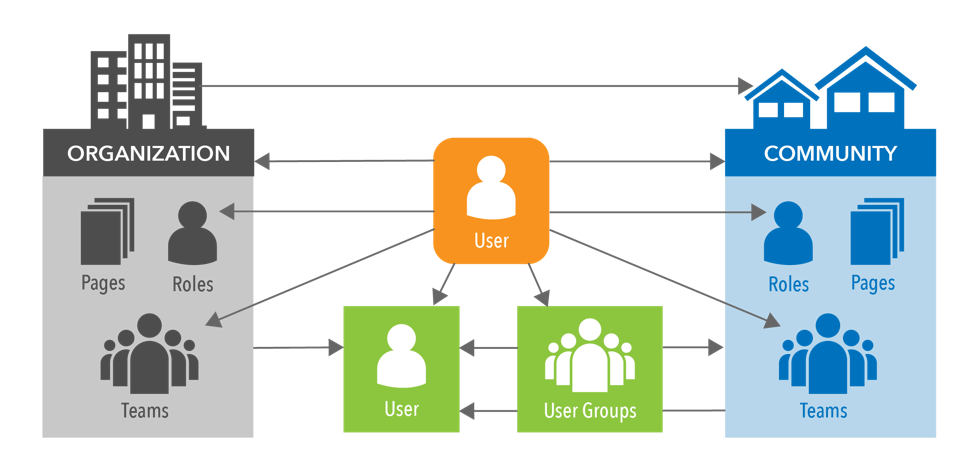
\includegraphics[width=1.0\linewidth]{liferay_structure}
	\caption{Model štruktúry a oprávnení portálového servera Liferay\cite{sezov2010portal}}
	\label{liferay_structure}
\end{figure}

\section{Portlety}
Základnou stavebnou jednotkou portálu v Liferay je portlet. Každá stránka portálu sa skladá z portletov, pričom každý portlet je v kontexte Liferay samostatná aplikácia. Užívateľ je schopný umiestňovať tieto portlety ľubovoľne po stránke a nastavovať im parametre.

Liferay obsahuje veľké množstvo vopred pripravených portletov, avšak jeho hlavná výhoda tkvie v možnosti rozšíriť ponuku týchto portletov o svoje vlastné. Jednotlivé stránky obsahujúce portlety (pages) je potom možné zaraďovať do lokalít (sites).

\section{Stránky}
Stránky sú stavebné elementy v Liferay ktoré obsahujú portlety. Podľa viditeľnosti stránok pre používateľov delíme stránky na:
\begin{description}
\item[Verejné stránky] - sú viditeľné aj pre užívateľov, ktorí nie sú registrovaný v systéme
\item[Privátne stránky] - vyžadujú sa určité oprávnenia, ktoré musí mať užívateľ priradené
\begin{itemize}
\item privátna stránka používateľa - len autor má k nej prístup
\item stránka používateľskej skupiny - ak je užívateľ priradený do tejto skupiny, má prístup na stránku
\item privátna stránka portálu - každý prihlásený používateľ má prístup na stránku
\end{itemize}
\end{description}

\section{Lokality}
Podstatným elementom Liferay sú lokality (Sites), ktoré pomáhajú vytvárať organizovanú štruktúru stránok a používateľov. Na základe nastavení lokality potom môžeme spravovať práva prístupu pre jednotlivých užívateľov. Liferay podporuje tri základné typy lokalít\cite{burska2016portlety}:
\begin{description}
\item[Otvorené (Open)] - ľubovoľný používateľ sa môže stať členom danej lokality, stačí keď si danú lokalitu nájde v zozname
\item[Na požiadanie (Retricted)] - členstvo používateľa v danej lokalite musí byť schválené
\item[Súkromné (Private)] - lokalita nie je viditeľná bežnému užívateľovi ani v zozname, jeho členstvo musí byť manuálne nastavené administrátorom
\end{description}
Z kapitoly \ref{liferay_users} však vieme, že lokality sú priradené organizácii a preto nastavenie oprávnení platí rovnako pre všetkých užívateľov spadajúcich pod danú organizáciu. Aby lokalita mohla užívateľom zobrazovať nejaký obsah, musí obsahovať aspoň jednu stránku.


\chapter{Modul časovej osy}
\section{Požiadavky}
Požiadavky na dizajn a funkcionalitu som vytvoril na základe konzultácií s vedúcim práce Radkom Ošlejškom.

Hlavnou úlohou časovej osy je
\begin{itemize}
\item zrozumiteľne zobraziť informáciu užívateľovi o aktuálne zvolenom časovom rozsahu
\item umožniť užívateľovi vybrať a neskôr upraviť časový rozsah pomocou vhodného nástroja
\end{itemize}

\section{Funkčné požiadavky}
Medzi funkčné požiadavky patria
\begin{itemize}
\item časová os si zistí možné časové ohraničenie volaním verejného API rozhrania cez REST
\item v prípade dát pribúdajúcich v reálnom čase bude mať užívateľ možnosť definovať správanie osy pri zmene týchto dát.
\item užívateľ bude informovaný vhodnou hláškou ak sa REST volanie nepodarí, alebo príde nevyhovujúca odpoveď
\item časovú os bude možné spustiť v móde \textit{LIVE} dát pričom sa bude meniť len horné ohraničenie. Dynamickosť dát bude zabezpečovať samotný modul pomocou periodických volaní API vždy po uplynutí vopred definovanej doby.
\end{itemize}

\section{Nefunkčné požiadavky}
Medzi nefunkčné požiadavky patria
\begin{itemize}
\item modul bude pracovať s časovými známkami, takže nebude závislý na časových pásmach
\item modul bude pozostávať z dvoch časových osí uložených nad sebou. Vrchná časová os bude vždy zobrazovať celé možné ohraničenie, zatiaľ čo spodná bude zobrazovať len práve zvolený výber.
\item definovanie správania časovej osy v prípade zmeny ohraničenia bude implementované pomocou zámkov. Bude možné zamkýnať obe strany časovej osy. Požiadavky na funkcionalitu zámkov sú opísané v sekcii \ref{sec:lockers}~\nameref{sec:lockers}.
\item modul bude implementovaný v aktuálnej verzii frameworku Angular, v súčasnosti sa jedná o verziu 5.2.8
\end{itemize}

\section{Funkcia zámkov}
\label{sec:lockers}
Zámky

\chapter{Angular framework}
Angular je open-source platforma od spoločnosti Google určená pre tvorbu jednostránkových front-end aplikácií. Využíva TypeScript ako odporúčaný programovací jazyk, ale je možné využiť aj JavaScript.

\section{TypeScript}
TypeScript je programovací jazyk vyvýjaný firmou Microsoft. Prvý krát bol oficiálne predstavený v roku 2012 a je označovaný ako "syntaktický cukor" pridaný do JavaScriptu, ktorý umožňuje využívať typovú kontrolu.

\subsection{Porovnanie s JavaScriptom}
JavaScript je dynamicky typovaný jazyk. To znamená, že typ premennej záleží na samotnej hodnote danej premennej. V jednotlivých fázach aplikácie teda môžeme do premennej priradiť hodnoty rôznych typov. To nám v istom smere poskytuje veľkú slobodu, ale zároveň vnáša istú mieru nepresnosti a neurčitosti do kódu, čo môže hlavne v rozsiahlych aplikáciách spôsobiť problémy so spoľahlivosťou.

\begin{lstlisting}
private example(): void {
  let attribute = 'some_string';
  console.log(typeof attribute); // nam vrati "string"
  attribute = 54;
  console.log(typeof attribute); // nam vrati "number"
}
\end{lstlisting}

TypeScript tvorí nadstavbu nad JavaScriptom. Výsledkom je teda kód, ktorý sa vo výsledku aj tak preloží len do JavaScriptu, avšak vďaka tomuto prekladu získame typovú kontrolu. Okrem toho nám niektoré editory podporujúce TypeScript dokážu navrhovať a zvýrazňovať syntax na základe vopred nadefinovaných typov. Pre vyššie uvedený kód by TypeScriptový prekladač skončil s chybou.

Typescript teda môžeme považovať za staticky typovaný jazyk, avšak výzkum Kalifornskej univerzity\cite{ray2014large} ukázal, že približne 50\% všetkých použitých atribútov v bežnom TypeScript kóde má deklarovaný typ \textit{any}, pre ktorý prekladač typovú kontrolu nevykonáva. Je teda na mieste úvaha, či môžeme považovať typovú kontrolu v TypeScripte za plnohodnotnú. Môj názor je, že pri dodržiavaní správnych postupov a zvyklostí pri programovaní je táto kontrola zmysluplná.

\printbibliography

%\printbibliography[heading=bibintoc] %% Print the bibliography.

\chapter{Inserting the index}
After using the \verb"\makeindex" macro and loading the
\texttt{makeidx} package that provides additional indexing
commands, index entries can be created by issuing the \verb"\index"
command. \index{dummy text|(}It is possible to create ranged index
entries, which will encompass a span of text.\index{dummy text|)}
To insert complex typographic material -- such as $\alpha$
\index{alpha@$\alpha$} or \TeX{} \index{TeX@\TeX} --
into the index, you need to specify a text string, which will
determine how the entry will be sorted. It is also possible to
create hierarchal entries. \index{vehicles!trucks}
\index{vehicles!speed cars}

After typesetting the document, it is necessary to generate the
index by running
\begin{center}%
  \texttt{texindy -I latex -C utf8 -L }$\langle$\textit{locale}%
  $\rangle$\texttt{ \jobname.idx}
\end{center}
from the command line, where $\langle$\textit{locale}$\rangle$
corresponds to the main locale of your thesis -- such as
\texttt{english}, and then typesetting the document again.

The \texttt{texindy} command needs to be executed from within the
directory, where the \LaTeX\ source file is located. In Windows,
the command line can be opened in a directory by holding down the
\textsf{Shift} key and by clicking the right mouse button while
hovering the cursor over a directory. Select the \textsf{Open Command
Window Here} option in the context menu that opens shortly
afterwards.

With online services -- such as Overleaf -- the commands are
executed automatically, although the locale may be erroneously
detected, or the \texttt{makeindex} tool (which is only able to
sort entries that contain digits and letters of the English
alphabet) may be used instead of \texttt{texindy}. In either case,
the index will be ill-sorted.

  \makeatletter\thesis@blocks@clear\makeatother
  \phantomsection %% Print the index and insert it into the
  \addcontentsline{toc}{chapter}{\indexname} %% table of contents.
  \printindex

\appendix %% Start the appendices.
\chapter{An appendix}
Here you can insert the appendices of your thesis.

\end{document}